\subsection{Results for $C_{DS}=0.0$}
The following results are for a run with the following input conditions:
\begin{longtable}[c]{A{3.0cm}  A{3.0cm}}
    \caption{Input list for $C_{DS}=0$ test}    \\  \hline
        \textbf{Parameter}      &       \textbf{Value}      \\  \hline
    \endfirsthead
    \caption{Input list for $C_{DS}=0$ test~(continued)}    \\  \hline
        \textbf{Parameter}      &       \textbf{Value}      \\  \hline
    \endhead
        $N$                 &   64      \\
        $t_{final}$         &   100.0   \\
        $C_{DS}$            &   0.0     \\
        $C_{BS}$            &   1.0     \\
\end{longtable}

\begin{figure}[H]
    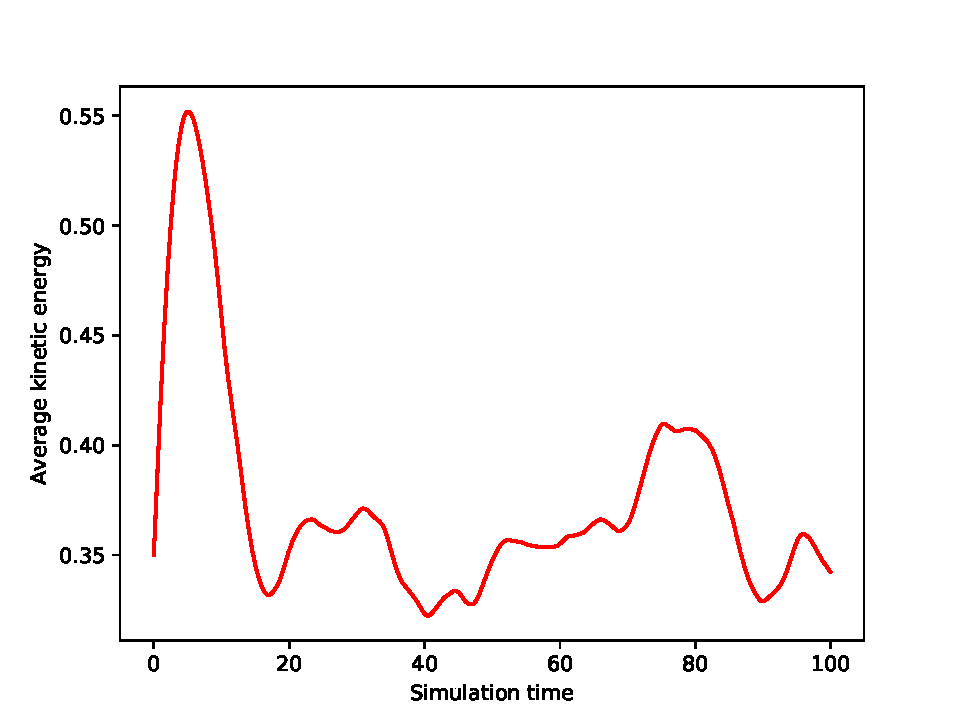
\includegraphics[height=0.4\textheight]{media/run-cds-00/average-ke-cds-00}
    \caption{Average kinetic energy versus simulation time}
\end{figure}

\begin{figure}[H]
    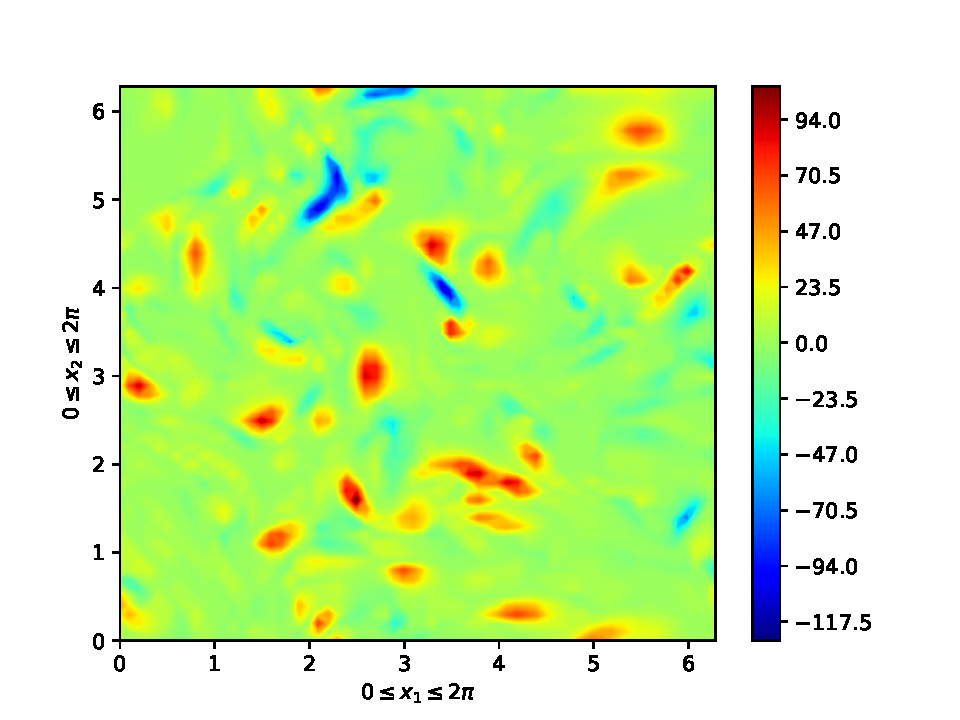
\includegraphics[height=0.4\textheight]{media/run-cds-00/A-term-enstrophy}
    \caption{$A_{\Omega}$ results at $z=32$}
\end{figure}

\begin{figure}[H]
    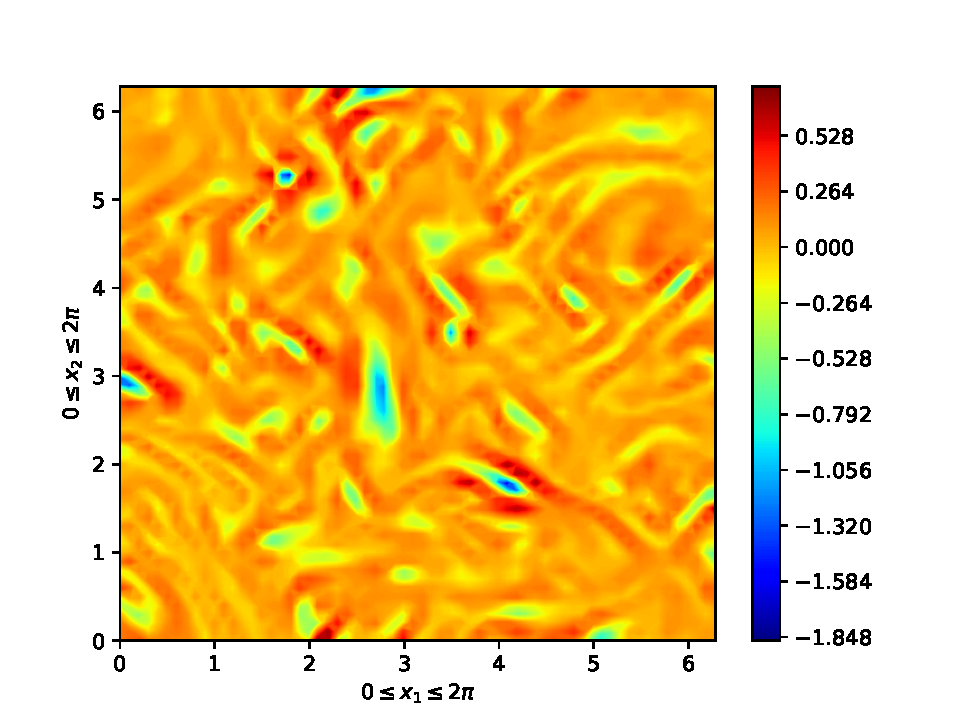
\includegraphics[height=0.4\textheight]{media/run-cds-00/C-term-enstrophy}
    \caption{$B_{\Omega}$ results at $z=32$}
\end{figure}

\begin{figure}[H]
    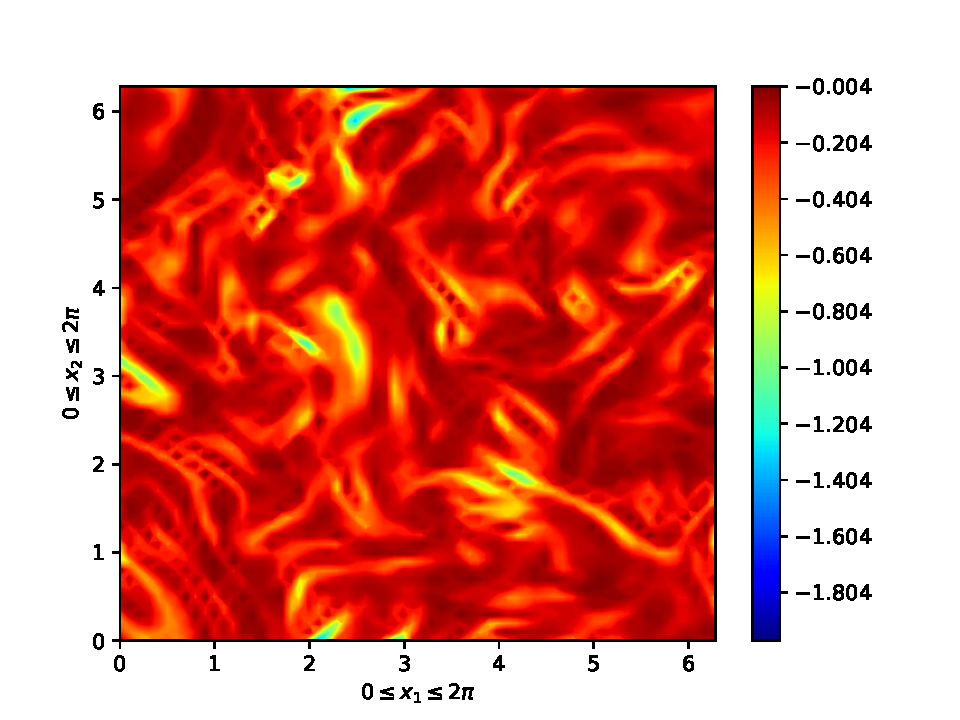
\includegraphics[height=0.4\textheight]{media/run-cds-00/D-term-enstrophy}
    \caption{$D_{\Omega}$ results at $z=32$}
\end{figure}

\begin{figure}[H]
    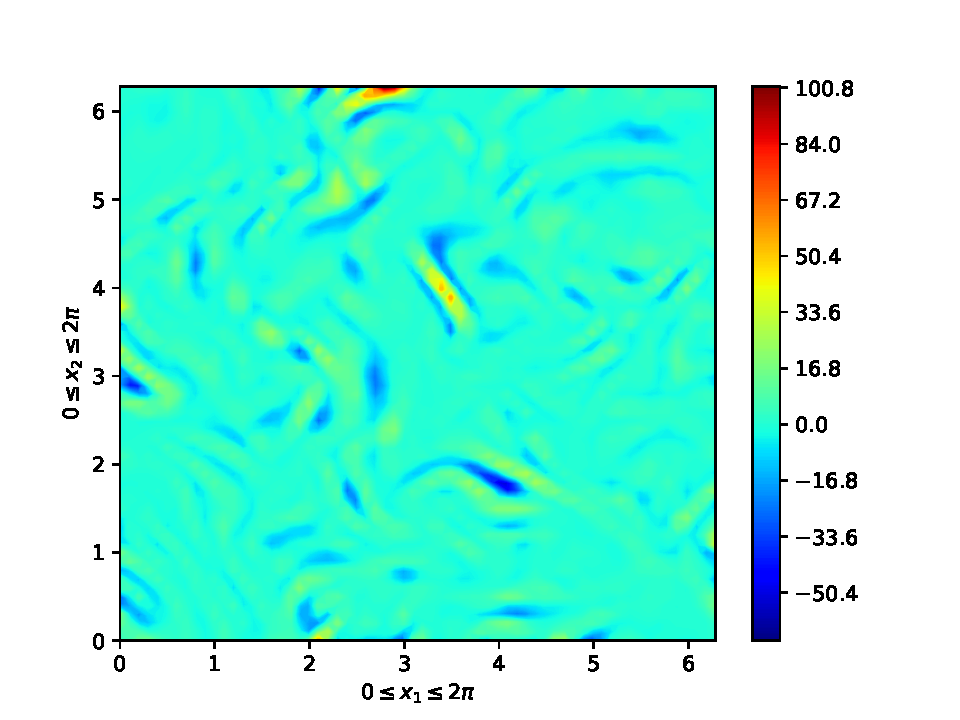
\includegraphics[height=0.4\textheight]{media/run-cds-00/SGS-transport-term-enstrophy}
    \caption{$\Pi_{\Omega}$ results at $z=32$}
\end{figure}

\begin{figure}[H]
    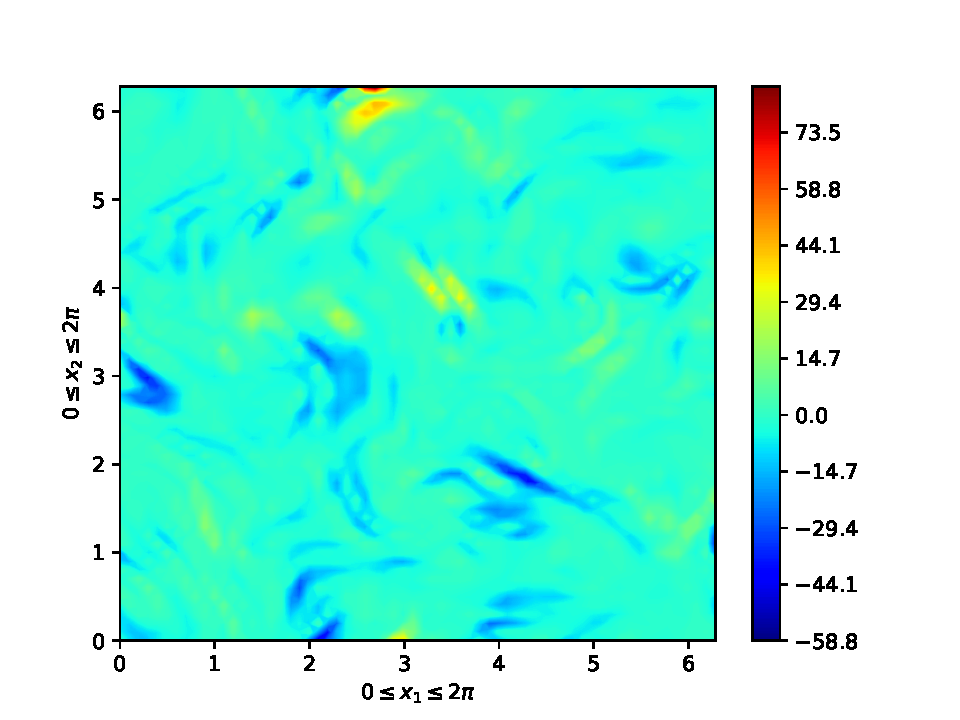
\includegraphics[height=0.4\textheight]{media/run-cds-00/SGS-production-term-enstrophy}
    \caption{$P_{\Omega}$ results at $z=32$}
\end{figure}
